\documentclass{article}
\usepackage{tikz, comment}
\usepackage{pifont}
\usepackage{fontspec, pgfplots}
\usetikzlibrary{arrows, decorations.markings, decorations.pathreplacing}
\begin{comment}
:Title: Not defined yet
:Tags: circumcenter;cross product;point of division formula;triple (scalar) product;moment
:Prob: 0.4746;0.4601;0.4468;0.4427;0.4348
:Author: Prof.Hu Ji-shan, HKUST
:Slug: No name yet

Description Here.........
\end{comment}
\begin{document}\centering 

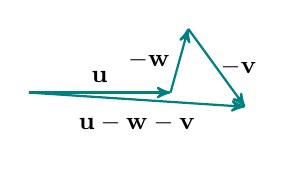
\begin{tikzpicture}[>=latex,xscale=.5*1.8, yscale=.5*1.8][font=\sf\small] 

\draw[teal, thick, ->, >=stealth'] (0, 0) -- (2, 0)node[black, above, midway, pos=0.5, xshift=0, yshift=0, scale=1]{$\bf u$}; %u

\begin{scope}[xshift=2cm,yshift=0cm]
\draw[teal, thick, ->, >=stealth'] (0, 0) -- (0.25, 0.9)node[black, left, midway, pos=0.5, xshift=0, yshift=0, scale=1]{$\bf -w$}; %-w

\begin{scope}[xshift=0.25cm,yshift=0.9cm]
\draw[teal, thick, ->, >=stealth'] (0, 0) -- (0.8, -1.1)node[black, right, midway, pos=0.5, xshift=-2, yshift=0, scale=1]{$\bf -v$}; %-v

\end{scope}

\end{scope}

\draw[teal, thick, ->, >=stealth'] (0, 0) -- ({2+0.25+0.8}, {0+0.9-1.1})node[black, below, midway, pos=0.5, xshift=0, yshift=-2, scale=1]{$\bf u - w - v$};

\end{tikzpicture}
\end{document}